\lab{Breadth-first Search}{Breadth-first Search}
\objective{
Shortest path problems are an important part of graph theory and network analysis.
Applications include finding the fastest way to drive between two points on the map, network routing, genealogy, automated circuit layout, and a variety of other problems.
In this lab we learn to represent graphs as adjacency dictionaries, implement a shortest-path algorithm based on a breadth-first search, and use the NetworkX package to solve a shortest path problem on a large actor-movie network.}

\section*{Adjacency Dictionaries} % ===========================================

Computers can represent mathematical graphs in various ways.
Graphs with very specific structures are often stored with specialized data structures, such as binary search trees.
More general graphs without structural constraints are usually represented with an \emph{adjacency matrix}, where each row and column of the matrix corresponds to a node in the graph, and the entries indicate connections between nodes.
Adjacency matrices are usually implemented in a sparse matrix format since only the entries corresponding to node connections are nonzero.

Another common graph data structure is an \emph{adjacency dictionary}, a dictionary with a key for each node in the graph.
The dictionary values list the nodes connected to the key node.
Adjacency dictionaries automatically gain the advantages of a sparse matrix format since they only store the actual node connections.
In Python, dictionaries are also much faster for lookup than matrices.

\begin{figure}[H] % simple graph, its adjacency matrix, and its adjacency dict.
\captionsetup[subfigure]{justification=centering}
\centering
\begin{subfigure}{.32\textwidth}
\centering
\begin{tikzpicture}[normalcircle/.style={draw,circle,minimum size=.75cm,fill=none,thick,node distance=1.5cm}]
    % Nodes
    \node[normalcircle] (A) [] {A};
    \node[normalcircle] (B) [above of=A] {B};
    \node[normalcircle] (C) [right of=B] {C};
    \node[normalcircle] (D) [below of=C] {D};
    % Edges
    \foreach \a/\b in {A/B,A/D,B/D,C/D} \draw[thick,-,>=stealth'] (\a) edge (\b);
\end{tikzpicture}
\end{subfigure}
%
\begin{subfigure}{.32\textwidth}
\centering
\begin{align*}
    \begin{blockarray}{ccccccc}
    & & \small\text{\textcolor{gray}{A}} & \small\text{\textcolor{gray}{B}} & \small\text{\textcolor{gray}{C}} & \small\text{\textcolor{gray}{D}} & \\
    \begin{block}{c[cccccc]}
    \small\text{\textcolor{gray}{A}} & & 0 & 1 & 0 & 1 & \topstrut\\
    \small\text{\textcolor{gray}{B}} & & 1 & 0 & 0 & 1 & \\
    \small\text{\textcolor{gray}{C}} & & 0 & 0 & 0 & 1 & \\
    \small\text{\textcolor{gray}{D}} & & 1 & 1 & 1 & 0 & \botstrut\\
    \end{block}\end{blockarray}
\end{align*}
\end{subfigure}
%
\begin{subfigure}{.32\textwidth}
\centering
\begin{align*}
\{\text{A}&:\ \{\text{B},\ \text{D}\},\\
  \text{B}&:\ \{\text{A},\ \text{D}\},\\
  \text{C}&:\ \{\text{D}\},\\
  \text{D}&:\ \{\text{A},\ \text{B},\ \text{D}\}\}
\end{align*}
\end{subfigure}
\caption{A simple unweighted graph (left), its adjacency matrix (middle), and its adjacency dictionary (right).
The graph is undirected, so the adjacency matrix is symmetric.
Note that the adjacency dictionary also encodes this behavior: since A and B are connected, B is in the set of values corresponding to the key A, and A is in the set of values corresponding to the key B.}
% There are eight $1$'s in the matrix, corresponding to $8$ total values in the dictionary.}
\label{fig:bfs-simple-graph_graph}
\end{figure}

\subsection*{Hash-based Data Structures} % ------------------------------------

A Python \li{set} is an unordered data type with no repeated elements.
The \li{set} class is implemented as a \emph{hash table}, meaning it uses \emph{hash values}---integers that uniquely identify an object---to organize its elements.
Roughly speaking, in order to access, add, or remove and object $x$ to a set, Python computes the hash value of $x$, and that value indicates where $x$ is (or should be). % (usually with the built-in \li{hash()} function)
In other words, there is only one place that $x$ could be; if it isn't in that place, it isn't in the set.
This implementation results in $O(1)$ lookup, insertion, and removal operations, an enormous improvement over the $O(n)$ search time for lists and the $O(\log{n})$ search time for sorted structures.
It is also why set elements are unique.

\begin{table}[H]
\begin{tabular}{r|l}
    Method & Description\\
    \hline
    \li{add()} & Add an element to the set if not already in the set.\\
    \li{remove()} & Remove the specified element from the set,\\
    & raising an error if the element is not in the set.\\
    \li{discard()} & Remove the specified element from the set without \\
    & raising an error if the element is not in the set.\\
    \li{pop()} & Remove and return an arbitrary set element.\\
    \li{union()} & Return all elements that are in either set as a new set.\\
    \li{intersection()} & Return all elements that are in both sets as a new set.\\
    \li{update()} & Perform an in-place union of a set with others.
\end{tabular}
\caption{Basic methods of the \li{set} class.}
\end{table}

\begin{lstlisting}
# Initialize a set. Note that repeats are not added.
>>> animals = {"cow", "cat", "dog", "mouse", "cow"}
>>> print(animals)
<<{'cow', 'dog', 'mouse', 'cat'}>>

>>> animals.add("horse")     # Add an object to the set.
>>> animals.remove("emu")    # Attempt to delete an object from the set,
<<KeyError: 'emu'>>              # resulting in an exception.

>>> animals.pop()            # Delete and return a random object from the set.
<<'dog'>>
>>> print(animals)
<<{'cat', 'mouse', 'cow', 'horse'}>>

# Add all of the elements of another set to this one.
>>> animals.update({"mouse", "velociraptor"})
>>> print(animals)
<<{'cat', 'mouse', 'velociraptor', 'cow', 'horse'}>>

# Intersect this set with another one.
>>> animals.intersection({"cat", "cow", "cheetah"})
<<{'cat', 'cow'}>>
\end{lstlisting}

\begin{warn} % hashable objects only
Elements of a \li{set} and keys (but not values) of a \li{dict} must be \emph{hashable}.
Mutable objects---lists, sets and dictionaries---are not hashable, so they are not allowed as set elements or dictionary key values.
This means that in order to represent a graph with an adjacency dictionary, each of the node labels should a string, a number, or some other hashable time.
\end{warn}

Dictionaries are similar to sets, except that elements in a dictionary are key-value pairs.
Keys in a dictionary must also be hashable, but values can be anything.
Because, like sets, lookup in a dictionary is very fast, they can be very useful for storing the results of a computation, so that it need only be done once.
The table below gives a quick review of dictionaries.

\begin{table}[H]
\begin{tabular}{r|l}
    Method & Description\\
    \hline
    \li{keys()} & Return an iterator for the dictionary's keys.\\
    \li{values()} & Return an iterator for the dictionary's values.\\
    \li{items()} & Return an iterator for the dictionary's items (key-value pairs).\\
    \li{pop()} & Remove and return a specified key from the dictionary.\\
    \li{update()} & Add or overwrite key-value pairs with those from a new dictionary.
\end{tabular}
\end{table}

\begin{lstlisting}
# Initialize a dictionary.
>>> classes = {"business": "A", "math": "A+", "visual arts": "B"}
>>> print(classes["math"])
<<A+>>

# Add a value indexed by 'science' and delete the 'business' keypair.
>>> classes["science"] = "A"
>>> classes.pop("business")  # Use pop() to remove.
<<A>>
>>> print(classes)
<<{'math': 'A+', 'visual arts': 'B', 'science': 'A'}>>

# Display the keys, values, and items.
>>> list(classes.keys())
<<['math', 'visual arts', 'science']>>
>>> classes.values()
<<dict_values(['A+', 'B', 'A'])>>
>>> for key, value in classes.items():
...   print(key, "=>", value)
...
<<math => A+
visual arts => B
science => A>>

# Add key-value pairs from another dictionary.
>>> classes.update({"cooking":"A+", "math": "C"})
>>> print(classes)
<<{'math': 'C', 'visual arts': 'B', 'science': 'A', 'cooking': 'A+'}>>

# Save time by pre-computing functions and storing results for quick lookup.
>>> f = lambda x: "My grade is " + x
>>> my_grades = {x:f(classes[x]) for x in ('math','science')}
>>> print(my_grades)
<<{'math': 'My grade is C', 'science': 'My grade is A'}>>
\end{lstlisting}

Figure \ref{fig:bfs-simple-graph_graph} is an example of a simple graph. The following code defines its adjacency dictionary.

\begin{lstlisting}
>>> adjacency_dictionary = {'A':{'B', 'D'},
                            'B':{'A', 'D'},
                            'C':{'D'},
                            'D':{'A', 'B', 'C'}}

# The nodes are stored as the dictionary keys.
>>> print(adjacency_dictionary.keys())
<<{'A', 'C', 'B', 'E', 'D'}>>

# The values are the nodes that the key is connected to.
>>> print(adjacency_dictionary['A'])
<<{'B', 'D'}>>            # A is connected to B and D.
\end{lstlisting}

% Problem 1: node, edge methods for Graph class (warmup with dictionaries)
\begin{problem}
Consider the following \li{Graph} class.
\begin{lstlisting}
class Graph:
    """A graph object, stored as an adjacency dictionary. Each node in the
    graph is a key in the dictionary. The value of each key is a set of
    the corresponding node's neighbors.

    Attributes:
        d (dictionary): the adjacency dictionary of the graph.
    """
    def __init__(self, adjacency):
        """Store the adjacency dictionary as a class attribute"""
        self.d = adjacency

    def __str__(self):
        """String representation: a view of the adjacency dictionary."""
        return str(self.d)
\end{lstlisting}
Add the following methods to this class.
\begin{enumerate}
\item \li{add_node(self, n)}: Add a node \li{n} to the graph.
\item \li{add_edge(self, u, v)}: Add an edge from node \li{u} to node \li{v} in the graph. Make sure to add the nodes if they are not already in the graph.
\item \li{remove_node(self, n)}: Remove the node \li{n} from the graph. Make sure to remove all connections to \li{n} as well.
Raise a \li{KeyError} if \li{n} is not in the graph.
\item \li{remove_edge(self, u, v)}: Remove the edge from node \li{u} to node \li{v} from the graph.
Raise a \li{KeyError}: if \li{u} or \li{v} are not in the graph, or if there is no edge between \li{u} and \li{v}.
\\(Hint: Dictionaries and sets already raise errors with certain inputs.)
\end{enumerate}
\end{problem}

\section*{Breadth-first Search}

Many of the most common problems that arise in graph theory require finding the shortest path between two nodes in the graph.
Doing so requires a way to strategically search the graph.
Two common searches are depth-first search (DFS) and breadth-first search (BFS).
The BFS strategy is typically better at finding shortest paths than the DFS strategy\footnote{\url{https://xkcd.com/761/}}.

To traverse a graph with a BFS, choose a starting node.
If the starting node is not the target node, explore each of the starting node's neighbors.
If none of the neighbors are the target, explore each of the neighbors' neighbors.
If none of those neighbors are the target, explore each of their neighbors.
Continue the process until the target is found.
Note that in this way, we explore the \emph{breadth} of the tree before going deeper each time.

In order to avoid common pitfalls, use the following data structures to keep track of visited and current nodes, as well as those marked to be visited.
\begin{enumerate}
  \item A list V - The nodes that have been visted (in the order that they were visited).
  \item A queue Q - The order in which to visit nodes.
  \item A set M (marked) - The nodes marked as visited, and marked for visitation.
\end{enumerate}

Recall that a \emph{queue} is a type of limited-access list.
Data is inserted to the back of the queue, but removed from the front.
At each level of the search, we add the neighbors of the current node to the back of Q if they aren't in M already.
This dictates the order in which the nodes are visited.
Note that Q enforces the 'breadth-first' nature of a BFS.
Another data structure, or a different order on the nodes, would result in a different search.

By creating M, a set to contain all nodes that have already been visited, or that are marked to be visited, we avoid visiting these nodes again.
Checking set membership is very fast, so this additional data structure has minimal impact on the program's speed (and is faster than checking the queue).

\begin{figure}[H] % Example of a breadth-first search.
\captionsetup[subfigure]{justification=centering}
\centering
\begin{subfigure}{.6\textwidth}
    \centering
    \begin{tikzpicture}[normalcircle/.style={draw,circle,minimum size=.75cm,fill=none,thick,node distance=1.5cm}]
    % Nodes
    \node[normalcircle] (A) [fill=red!20] {A};
    \node[normalcircle] (B) [above of=A] {B};
    \node[normalcircle] (C) [right of=B] {C};
    \node[normalcircle] (D) [below of=C] {D};
    % Edges
    \foreach \a/\b in {A/B,A/D,B/D,C/D} \draw[thick,-,>=stealth'] (\a) edge (\b);
    \end{tikzpicture}
\end{subfigure}
%
\begin{subfigure}{.39\textwidth}
    \Large\begin{tabular}{r|l}
    $V$ & \textcolor{white}{A B C D} \\ \hline
    $Q$ & \textcolor{red}{A} \\ \hline
    $M$ & A \\
    \end{tabular}
\end{subfigure}
\\\vspace{20px}
\begin{subfigure}{.6\textwidth}
    \centering
    \begin{tikzpicture}[normalcircle/.style={draw,circle,minimum size=.75cm,fill=none,thick,node distance=1.5cm}]
    % Nodes
    \node[normalcircle] (A) [fill=blue!20] {A};
    \node[normalcircle] (B) [fill=red!20, above of=A] {B};
    \node[normalcircle] (C) [right of=B] {C};
    \node[normalcircle] (D) [fill=red!20, below of=C] {D};
    % Edges
    \foreach \a/\b in {B/D,C/D} \draw[thick,-,>=stealth'] (\a) edge (\b);
    \foreach \a/\b in {A/B,A/D} \draw[red!80,thick,->,>=stealth',line width=1.5pt] (\a) edge (\b);
    \end{tikzpicture}
\end{subfigure}
%
\begin{subfigure}{.39\textwidth}
    \Large\begin{tabular}{r|l}
    $V$ & \textcolor{blue}{A} \textcolor{white}{B C D} \\ \hline
    $Q$ & \textcolor{red}{B D} \\ \hline
    $M$ & A B D \\
    \end{tabular}
\end{subfigure}
\\\vspace{20px}
\begin{subfigure}{.6\textwidth}
    \centering
    \begin{tikzpicture}[normalcircle/.style={draw,circle,minimum size=.75cm,fill=none,thick,node distance=1.5cm}]
    % Nodes
    \node[normalcircle] (A) [fill=blue!20] {A};
    \node[normalcircle] (B) [fill=blue!20, above of=A] {B};
    \node[normalcircle] (C) [right of=B] {C};
    \node[normalcircle] (D) [fill=red!20, below of=C] {D};
    % Edges
    \foreach \a/\b in {A/B,A/D,B/D,C/D} \draw[thick,-,>=stealth'] (\a) edge (\b);
    \end{tikzpicture}
\end{subfigure}
%
\begin{subfigure}{.39\textwidth}
    \Large\begin{tabular}{r|l}
    $V$ & \textcolor{blue}{A B} \textcolor{white}{C D}\\ \hline
    $Q$ & \textcolor{red}{D} \\ \hline
    $M$ & A B D \\
    \end{tabular}
\end{subfigure}
\\\vspace{20px}
\begin{subfigure}{.6\textwidth}
    \centering
    \begin{tikzpicture}[normalcircle/.style={draw,circle,minimum size=.75cm,fill=none,thick,node distance=1.5cm}]
    % Nodes
    \node[normalcircle] (A) [fill=blue!20] {A};
    \node[normalcircle] (B) [fill=blue!20, above of=A] {B};
    \node[normalcircle] (C) [fill=red!20, right of=B] {C};
    \node[normalcircle] (D) [fill=blue!20, below of=C] {D};
    % Edges
    \foreach \a/\b in {A/B,A/D,B/D} \draw[thick,-,>=stealth'] (\a) edge (\b);
    \draw[red!80,thick,->,>=stealth',line width=1.5pt] (D) edge (C);
    \end{tikzpicture}
\end{subfigure}
%
\begin{subfigure}{.39\textwidth}
    \Large\begin{tabular}{r|l}
    $V$ & \textcolor{blue}{A B D} \\ \hline
    $Q$ & \textcolor{red}{C} \\ \hline
    $M$ & A B D C \\
    \end{tabular}
\end{subfigure}
\caption{To start a breadth-first search from node A to node C, put A in the visit queue $Q$ and mark it by adding it to the set $M$.
Pop A off the queue and ``visit'' it by adding A to the visited list $V$ and the neighboring nodes B and D to $Q$.
Then visit B, but do not add anything to $Q$ because all of the neighbors of B are already marked.
Finally, visit D, at which point the target node C is located because it is adjacent to D.
Visiting C is optional at this point.
}
\label{fig:bfs-example}
\end{figure}

% Problem 2: general BFS
\begin{problem}
Write a \li{traverse()} method for the \li{Graph} class that accepts a starting node and (optionally) a target node.
Start from the specified node and proceed until the target is found.
If no target is specified, proceed until all nodes in the graph have been visited.
Return the list of visited nodes.
If the starting node is not in the graph's adjacency dictionary, raise a \li{KeyError}.
\end{problem}

\section*{Shortest Paths via BFS} % ===========================================

In a BFS, as few neighborhoods are explored as possible before finding the target.
At each neighborhood, the minimal path is marked from the source node, until the target node is encountered.
Therefore, the path taken to get to the target must be the shortest path.

Examine again the graph in Figure \ref{fig:bfs-example}.
The shortest path from $A$ to $C$ starts at $A$, goes to $D$, and ends at $C$.
During a BFS, $D$ is visited because it is one of $A$'s neighbors, and $C$ is visited because it is one of $D$'s neighbors.
If we knew programmatically that $A$ was the node that visited $D$, and that $D$ was the node that visited $C$, we could retrace our steps to reconstruct the search path.

To implement this idea, initialize a dictionary before starting the BFS.
When a node is added to the visit queue, add a key-value pair with the visiting node as the key, and the added node as the value.
When the target node is found, step through the dictionary until arriving at the starting node, recording each step.

\begin{figure}[H] % Example of a breadth-first search.
\centering
\begin{tikzpicture}[normalcircle/.style={draw,circle,minimum size=.75cm,fill=none,thick,node distance=1.5cm}]
% Nodes
\node[normalcircle] (A) [fill=blue!20] {A};
\node[normalcircle] (B) [fill=blue!20, above of=A] {B};
\node[normalcircle] (C) [fill=blue!20, right of=B] {C};
\node[normalcircle] (D) [fill=blue!20, below of=C] {D};
% Edges
\draw[thick,-,>=stealth'] (B) edge (D);
\foreach \a/\b in {C/D,D/A,B/A} \draw[green!80,thick,->,>=stealth',line width=1.5pt] (\a) edge (\b);
\end{tikzpicture}
\caption{In the breadth-first search from Figure \ref{fig:bfs-example}, nodes B and D were marked while visiting node A, and node C was marked while visiting node D (this is same as reversing the red arrows in Figure \ref{fig:bfs-example}).
Thus the ``visit path'' from C to A is $\text{C}\rightarrow\text{D}\rightarrow\text{A}$, so the shortest path from A to C is $[$A, D, C$]$.}
\label{fig:bfs-shortest-path}
\end{figure}

\begin{problem}
Add a method to the \li{Graph} class that accepts a start node and a target node.
Begin at the specified starting node and proceed until the target is found.
Return a list containing the node values in the shortest path from the start to the target (including the endpoints).
If either of the inputs are not in the graph, raise a \li{KeyError}.
\end{problem}

\section*{Shortest Paths via NetworkX} % ======================================

\emph{NetworkX} is a Python package for creating, manipulating, and exploring large graphs.
It contains a \li{Graph} object constructor as well as methods for adding nodes and edges to the graph.
It also has methods for interpreting information about the graph and its structure from certain types of Python objects.

A node can be an int, a string, or a Python object, and an edge can be weighted or unweighted.
There are several ways to add nodes and edges to the graph, some of which are listed below.

\begin{table}[H]
\centering
\begin{tabular}{r|l}
    Method & Description\\
    \hline
    \li{add_node()} & Add a single node to the graph.\\
    \li{add_nodes_from()} & Add a list of nodes to the graph.\\
    \li{add_edge()} & Add an edge between two nodes.\\
    \li{add_edges_from()} & Add a list of edges to the graph.
\end{tabular}
\end{table}

\begin{lstlisting}
# Create a graph object using networkX using a known dictionary.
>>> import networkx as nx
>>> adjacency_dictionary = {'A':{'B', 'D'}, # The graph from earlier.
                            'B':{'A', 'D'},
                            'C':{'D'},
                            'D':{'A', 'B', 'C'}}
>>> nx_graph = nx.Graph(adjacency_dictionary)

# Access the nodes and edges.
>>> print(nx_graph.nodes())
<<['A', 'B', 'C', 'D']>>

>>> print(nx_graph.edges())
<<[('A', 'D'), ('A', 'B'), ('B', 'D'), ('C', 'D')]>>

>>> nx_graph.add_node('A')
>>> nx_graph.add_node('E')
>>> nx_graph.add_edge('A', 'F') # Node 'F' is added to the graph.
>>> nx_graph.add_edges_from([('A', 'E')])

# Access the nodes and edges.
>>> print(nx_graph.nodes())
<<['A', 'B', 'C', 'D', 'E', 'F']>>

>>> print(nx_graph.edges())
<<[('A', 'D'), ('A', 'B'), ('A', 'F'), ('A', 'E'), ('B', 'D'), ('C', 'D')]>>

# Small graphs can be visualized with nx.draw().
>>> from matplotlib import pyplot as plt
>>> nx.draw(nx_graph)
>>> plt.show()
\end{lstlisting}

\subsection*{The Kevin Bacon Problem} % ---------------------------------------

\href{http://oracleofbacon.org/help.php}{\emph{The 6 Degrees of Kevin Bacon}} is a vintage parlor game.
The game is played by naming an actor, then trying to find a chain of actors that have worked with each other leading to Kevin Bacon.
For example, Samuel L. Jackson was in the film \emph{Captain America: The First Avenger} with Peter Stark, who was in \emph{X-Men: First Class} with Kevin Bacon.
Thus Samuel L. Jackson has a \emph{Bacon number} of $2$.
Any actors who have been in a movie with Kevin Bacon have a Bacon number of $1$.
\begin{figure}
\centering
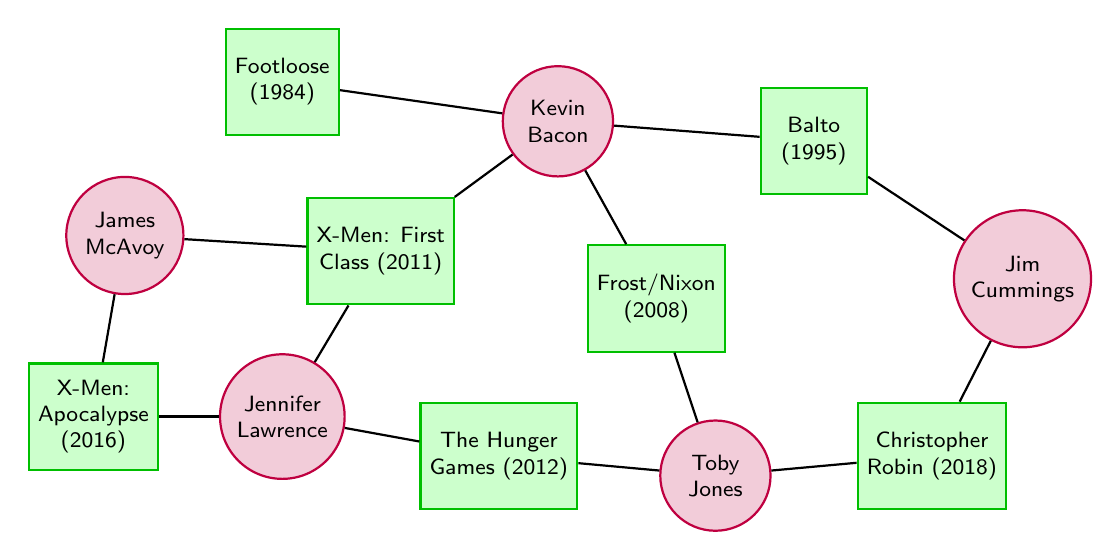
\begin{tikzpicture}
% Set styles for Actor and Movie nodes
\tikzstyle{Actor}=[thick,circle,draw=purple,fill=purple!20!,font=\sffamily\footnotesize,align=center,minimum size=1.4cm]
\tikzstyle{Movie}=[thick,rectangle,draw=green!75!black,fill=green!20!,font=\sffamily\footnotesize,align=center,minimum height=1.35cm,minimum width=1.35cm]
% Nodes
\foreach [count=\i] \x/\y/\t/\n in {
    0/1.25/Kevin\\Bacon/Actor,
    5.9/-.75/Jim\\Cummings/Actor,
    2/-3.25/Toby\\Jones/Actor,
    -3.5/-2.5/Jennifer\\Lawrence/Actor,
    -5.5/-.2/James\\McAvoy/Actor,
    3.25/1/{Balto\\(1995)}/Movie,
    4.75/-3/{Christopher\\Robin (2018)}/Movie,
    1.25/-1/{Frost/Nixon\\(2008)}/Movie,
    .-.75/-3/{The Hunger\\Games (2012)}/Movie,
    -2.25/-.4/{X-Men: First\\Class (2011)}/Movie,
    -5.9/-2.5/{X-Men:\\Apocalypse\\(2016)}/Movie,
    -3.5/1.75/{Footloose\\(1984)}/Movie}
  \node[\n] at (\x,\y) (v\i) {\t};
% Edges
\foreach \i/\j in {1/6, 2/6, 2/7, 3/7, 1/8, 3/8, 3/9,
                   4/9, 1/10, 4/10, 5/10,4/11,5/11,1/12}
  \draw[thick] (v\i) edge (v\j);
\end{tikzpicture}
\caption{A \textbf{very} small subset of the data from \texttt{movieData.txt}.
Each of the actors shown have a Bacon number of $1$ because they have all been in a movie with Kevin Bacon.
Every cast member of \emph{The Hunger Games} has a Bacon number of at most $2$ because of the paths through Jennifer Lawrence or Toby Jones.}
\end{figure}

\begin{problem} % MovieGraph.__init__()
Write a \li{MovieGraph} class to solve the Kevin Bacon problem.

The file \texttt{movieData.txt} contains data from about 13,000 movies.
A single movie is listed on each line, followed by a sequence of actors that starred in it.
The movie title and actors' names are separated by a \li{/} character.
The actors are listed by last name first, followed by their first name.

Implement the constructor of \li{MovieGraph}.
Accept a filename to read data from, and store the collection of values (the actors) as a class attribute, avoiding duplicates.
Create a networkX \li{Graph} and store it as another class attribute.
Note that in the graph, actors only have movies as neighbors, and movies only have actors as neighbors.
\\(Hint: recall the \li{split()} method for strings.)

\end{problem}

\begin{warn}
Because of the size of the dataset, \textbf{do not} attempt to visualize the graph in Problem 4 with \li{nx.draw()}.
The visualization tool in NetworkX is only effective on relatively small graphs.
In fact, graph visualization in general remains a challenging and ongoing area of research.
\end{warn}

NetworkX is equipped with a variety of methods to analyze graphs.

\begin{lstlisting}
# Verify nx_graph has a path from 'C' to 'E'.
>>> nx.has_path(nx_graph, 'C', 'E')
<<True>>

# The shortest_path method is implemented with a
# bidirectional BFS (starting from both ends).
>>> nx.shortest_path(nx_graph, 'C', 'E')
['C', 'A', 'E']
\end{lstlisting}

\begin{problem}
Write a method for the \li{MovieGraph} class that accepts source and target values (actors' names).
Set Kevin Bacon as the default target.
Return a list with the shortest path from the source to the target, and the number of actors in the list.
Note that this is different than the number of entries in the shortest path list, since movies do not contribute.
If either input is not an actor's name, raise a \li{ValueError}.
\begin{lstlisting}
>>> movie_graph = MovieGraph("movieData.txt")
>>> movie_graph.path_to_actor("Jackson, Samuel L.")
<<['Jackson, Samuel L.', 'Captain America: The First Avenger', 'Stark,
Peter', 'X-Men: First Class', 'Bacon, Kevin'], 2>>
\end{lstlisting}
\label{prob:actor_path}
\end{problem}

\begin{problem} % Individual and average Bacon numbers
Add a method to the \li{MovieGraph} class to calculate the average path length across all of the actors in the collection to the target (not including movies).
Set Kevin Bacon as the default target.
Use \li{plt.hist()} to plot the distribution of path lengths and return the average path length.
\\(Hint: The \li{path_to_actor()} method from Problem \ref{prob:actor_path} is not the most efficient way of doing this.
Also, consider how \li{bins} affects \li{plt.hist()})
\end{problem}

As an aside, the prolific \href{https://en.wikipedia.org/wiki/Erd%C5%91s_number}{Paul Erd\H{o}s} is considered the Kevin Bacon \href{https://xkcd.com/599/}{of the mathematical community}.
Someone with an ``Erd\H{o}s number'' of $2$ co-authored a paper with someone who co-authored a paper with Paul Erd\H{o}s.

\newpage

\section*{Additional Material} % ==============================================

\subsection*{Depth-first Search} % --------------------------------------------

% TODO: Revise this section. Need a (good) picture of a DFS, compared to a BFS.

A \emph{depth-first search} (DFS) takes the opposite approach of a breadth-first search.
Instead of checking all neighbors of a single node before moving, on, it checks the first neighbor, then their first neighbor, then their first neighbor, and so on until reaching a leaf node.
Then the algorithm back tracks to the previous node and checks its second neighbor.
The DFS method was originally developed as a strategy for solving mazes.
While a DFS is sometimes more useful than a BFS, a BFS is usually better\footnote{\url{https://xkcd.com/761/}} at finding the shortest path.

Consider adding a keyword argument to the \li{traverse()} method of the \li{Graph} class that specifies whether to use a BFS (the default) or a DFS.
This can be done by changing a single line of the BFS code.

\subsection*{Improvements to the MovieGraph Class} % -------------------------
% This doesn't really work anymore, since it's not a 'bacon number,' but rather a 'path to actor' or 'average number.'
Consider adding a \li{center_of_the_universe()} method in the \li{MovieGraph} class.
This should plot the distribution of average numbers and return the 'center of the universe,' or the actor to whom all other actors are most closely connected.
This can be found by returning the actor with the lowest average path length from all other actors.

\subsection*{More NetworkX}

The following are interesting methods that may be of use in further graph analysis.

\begin{table}[H]
\centering
\begin{tabular}{r|l}
    Function & Description\\
    \hline
    \li{adjacency_matrix()} & Returns the adjacency matrix as a SciPy sparse matrix.\\
    \li{dijkstra_path()} & Returns the shortest path from a source to a target in a weighted graph.\\
    \li{has_path()} & Returns \li{True} if the graph has a path from a source to a target.\\
    \li{prim_mst()} & Returns a minimum spanning tree for a weighted graph.\\
    \li{shortest_path()} & Returns the shortest path from a source to a target.
\end{tabular}
\end{table}
